
%(BEGIN_QUESTION)
% Copyright 2014, Tony R. Kuphaldt, released under the Creative Commons Attribution License (v 1.0)
% This means you may do almost anything with this work of mine, so long as you give me proper credit

Calculate all voltages and all currents in this transformer circuit, assuming the resistor in the primary side of the circuit drops 9 volts:

$$\includegraphics[width=15.5cm]{i01270x01.eps}$$

\begin{itemize}
\item{} $V_{source}$ = 
\item{} $V_{primary}$ = 
\item{} $V_{secondary}$ = 
\item{} $I_{primary}$ = 
\item{} $I_{secondary}$ = 
\end{itemize}

\vfil 

\underbar{file i01270}
\eject
%(END_QUESTION)





%(BEGIN_ANSWER)

This is a graded question -- no answers or hints given!

%(END_ANSWER)





%(BEGIN_NOTES)

\begin{itemize}
\item{} $V_{source}$ = 12.56 volts 
\item{} $V_{primary}$ = 3.56 volts
\item{} $V_{secondary}$ = 12.0 volts
\item{} $I_{primary}$ = 2.25 amps
\item{} $I_{secondary}$ = 0.667 amps
\end{itemize}

%INDEX% Electronics review: transformer ratios

%(END_NOTES)


